\documentclass[11pt]{article}

\usepackage{float}
\usepackage{fullpage}
\usepackage{times}
\usepackage[utf8]{inputenc}
\usepackage[T1]{fontenc}
\usepackage[english]{babel}
\usepackage{amssymb}
\usepackage{parskip}
\usepackage{url}
\usepackage{graphicx}

\begin{document}

\title{COMP512 - Distributed Systems \\ Deliverable III}
\author{
  Vincent Foley-Bourgon <vincent.foley-bourgon@mail.mcgill.ca> \\
  Carol Morneau <carol.morneau@mail.mcgill.ca>
}
\date{November 2013}

\maketitle

\tableofcontents

\section{Introduction}

This third deliverable is the culmination of the implementation of a
distributed reservation system.  The main features of our system are:

\begin{itemize}
  \item The middleware and three resource managers are independent and
    can be executed on different machines;
  \item The client, middleware and resource managers communicate
    through the Java RMI protocol;
  \item Data items are protected by a smart lock manager;
  \item Data in the resource managers is persisted to disk using a
    shadowing scheme;
  \item The system implements a two-phase commit protocol that makes
    it resilient to crashes;
  \item The client and resource managers have been extended to allow
    crashing at predefined points;
  \item A smart set of Makefile rules allow the different parts of the
    system to be started with minimal hassle.
\end{itemize}

This report will discuss these features, the general architecture of
the system, the implementation issues that were encountered during
development and the solutions we put in place, the performance
characteristics of the application and some diagrams showing how the
system handles different scenarios.


\section{RMI}

All interactions between the different software components is done
through the Java RMI protocol.  Figure~\ref{fig:rmi} illustrates how
the different components and registries are linked.  (One detail that
is not shown in this diagram is that for recovery purpose, resource
managers can obtain a reference to the middleware.  More information
on this case is available in the {\it Two-Phase Commit} section.)

The middleware and the resource managers each have their own, separate
registries.  The clients obtain a reference to the middleware by
querying the middleware's registry and the middleware obtains
references to the three resource managers by querying their respective
registries.  When executing the system, it is important to first start
the resource managers, then the middleware and finally the clients.

For more information concerning the RMI architectural design, please
consult deliverable I's report.

\begin{figure}[H]
  \caption{RMI System Architecture}
  \label{fig:rmi}

  \begin{center}
    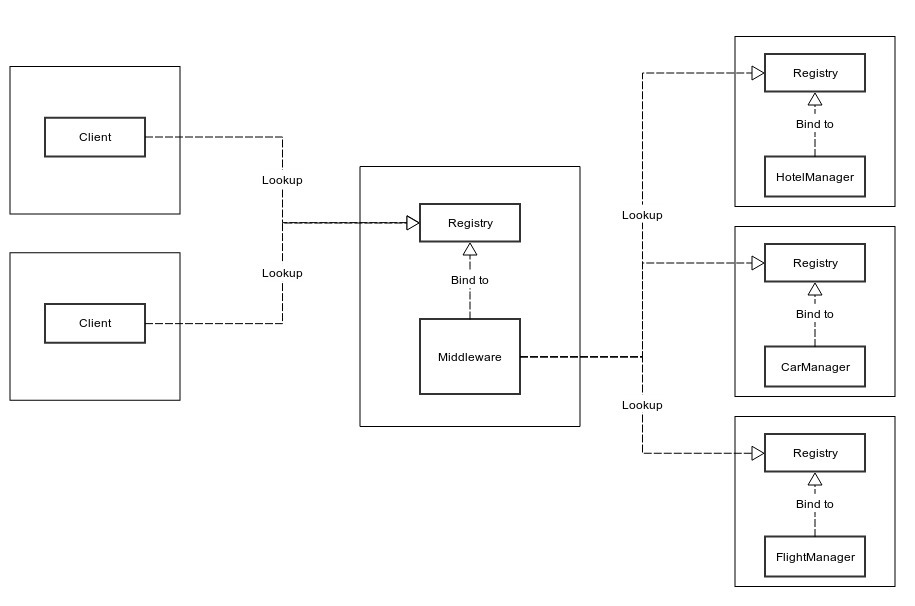
\includegraphics[scale=0.5]{rmi.jpg}
  \end{center}
\end{figure}



\section{Architecture}

In this section, we will give a general overview of the application's
architecture.  We will also describe the details of some components
that we feel deserve further explanations.

\subsection{Overview}

Figure~\ref{fig:architecture} shows the high-level architecture of the
application.  To keep the diagram light, we've included only a single
resource manager.

\begin{figure}[H]
  \caption{Global architecture}
  \label{fig:architecture}

  \begin{center}
    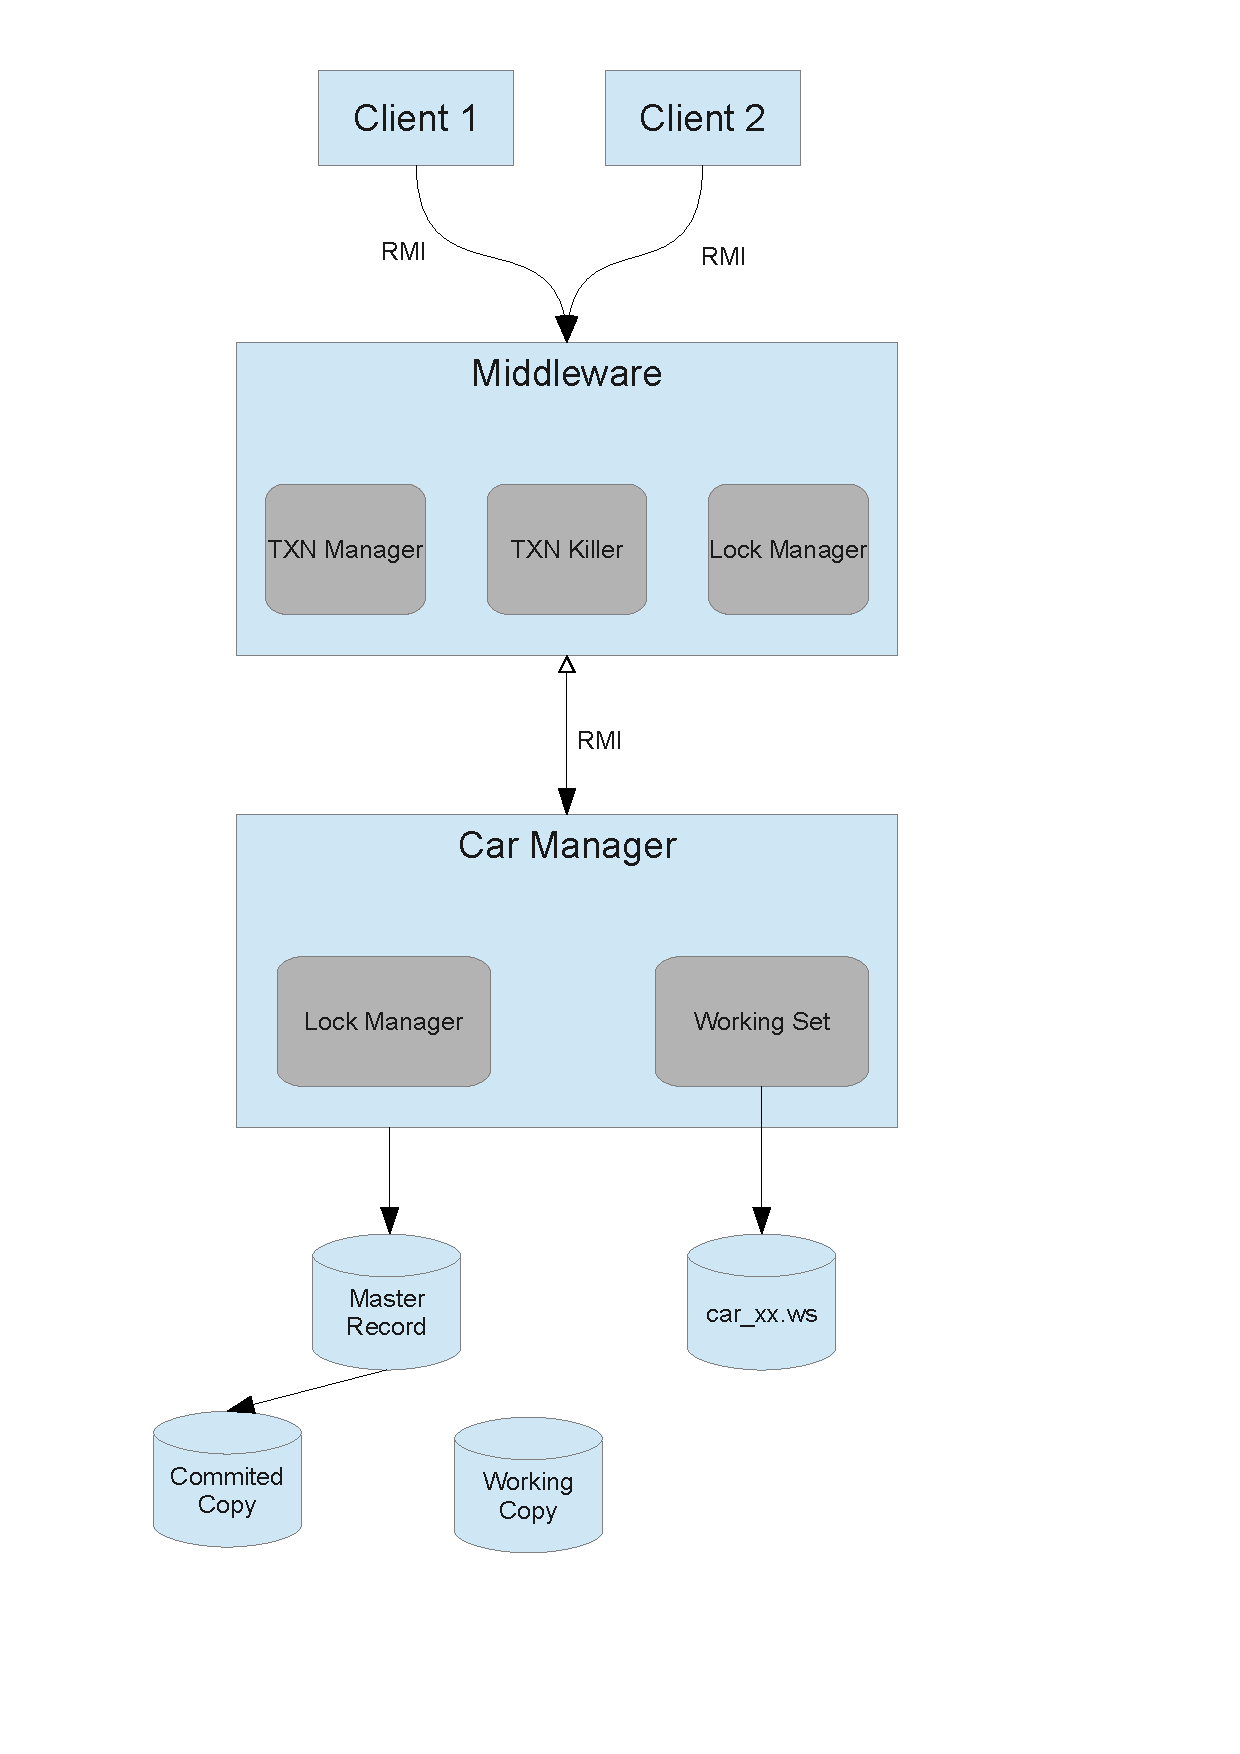
\includegraphics[scale=0.5]{architecture.pdf}
  \end{center}
\end{figure}

Although it is said that a picture is worth a thousand words, we will
take the liberty of explaining a few details that may not be evident
from the diagram alone.

\begin{itemize}
  \item The double RMI arrow link between the middleware and the
    resource manager is meant to convey that the resource manager does
    not always know about the middleware; only when it needs to
    recover from a crash do we give it a reference to the middleware,
    so that it can perform a query to know how what to do with
    transactions inside the persistent working set.
  \item The {\it car\_xx.ws} file is created during the first phase of
    the two-phase commit (in the {\it prepare} method) and is deleted
    at the end of the second phase.  It contains a copy of the
    resource manager's working set.
  \item The data items of the resource manager are persisted in two
    files: {\it cardb.0} or {\it cardb.1}.  A third file, the master
    record {\it cardb.mr}, contains a link to the currently committed
    copy of the database.  All these files are located in {\it
      /tmp/Group5/}.
  \item The middleware contains a lock manager because it handles the
    customer data items; we've omitted the data persistence entities
    in the figure to keep the diagram simpler.
\end{itemize}


\subsection{Working Set}

The {\it WorkingSet} class allows a transaction to perform different
actions without writing directly into the RMs' hash tables.  Each
resource manager (including the middleware) has one working set.  A
{\it WorkingSet} maintains three hash maps:

\begin{itemize}
  \item A table mapping transaction IDs to a vector of commands;
  \item A table mapping transaction IDs to a vector of item descriptions;
  \item A table mapping an item description to the new, modified state
    of the item.
\end{itemize}

As a client performs write actions on a data item, a symbolic
representation of those commands is appended to the first hash table,
and the state of the object's copy in the third hash table is updated.
Reads return values from the third hash table.

Once the client commits his transaction, the commands are executed
sequentially, thus modifying the state of the object inside the RM.
When a transaction is aborted, the entries for the transaction ID are
simply dropped from the hash tables.

The two types of commands we store are:

\begin{itemize}
\item {\it CommandPut} describing a write/modify action in a RM's hash
  table;
\item {\it CommandDelete} describing a delete action in a RM's hash
  table.
\end{itemize}

\subsection{Transaction manager}

The Transaction Manager is a singleton object that is in charge of
transactions.  Notably, it is in charge of the two-phase commit
protocol.

The transaction manager maintains multiple hash tables:

\begin{itemize}
  \item A table mapping transaction IDs to their two-phase commit
    status (NOTCOMMITTED, PHASE1, or PHASE2);
  \item A table mapping transaction IDs to a vector of the resource
    managers that they are involved with;
  \item A table mapping transaction IDs to their last action time
    (used for killing idle transactions);
  \item A table mapping transaction IDs to whether they should be
    committed or aborted.
\end{itemize}

During the two-phase commit process, the transaction manager is
marshalled to disk to allow transactions to resume their commit
process should the middleware crash and recover.  After the two-phase
commit, the transaction manager copy on disk is deleted.


\subsection{Transaction killer}

In a separate thread, we run a transaction killer, a singleton object
that inspects the time-to-live values of the active transactions.  If
a thread has been idle for more than a predefined number of seconds,
the thread will be aborted.



\section{Two-Phase Commit}

As in the architecture section, figure~\ref{fig:2pc} shows with a
high-level flow diagram of how a two-phase commit proceeds from the
point of view of a resource manager and figure~\ref{fig:2pc-mw} shows
the two-phase commit process from the point of view of the middleware.

\begin{figure}[H]
  \caption{Two-phase commit (resource manager view)}
  \label{fig:2pc}

  \begin{center}
    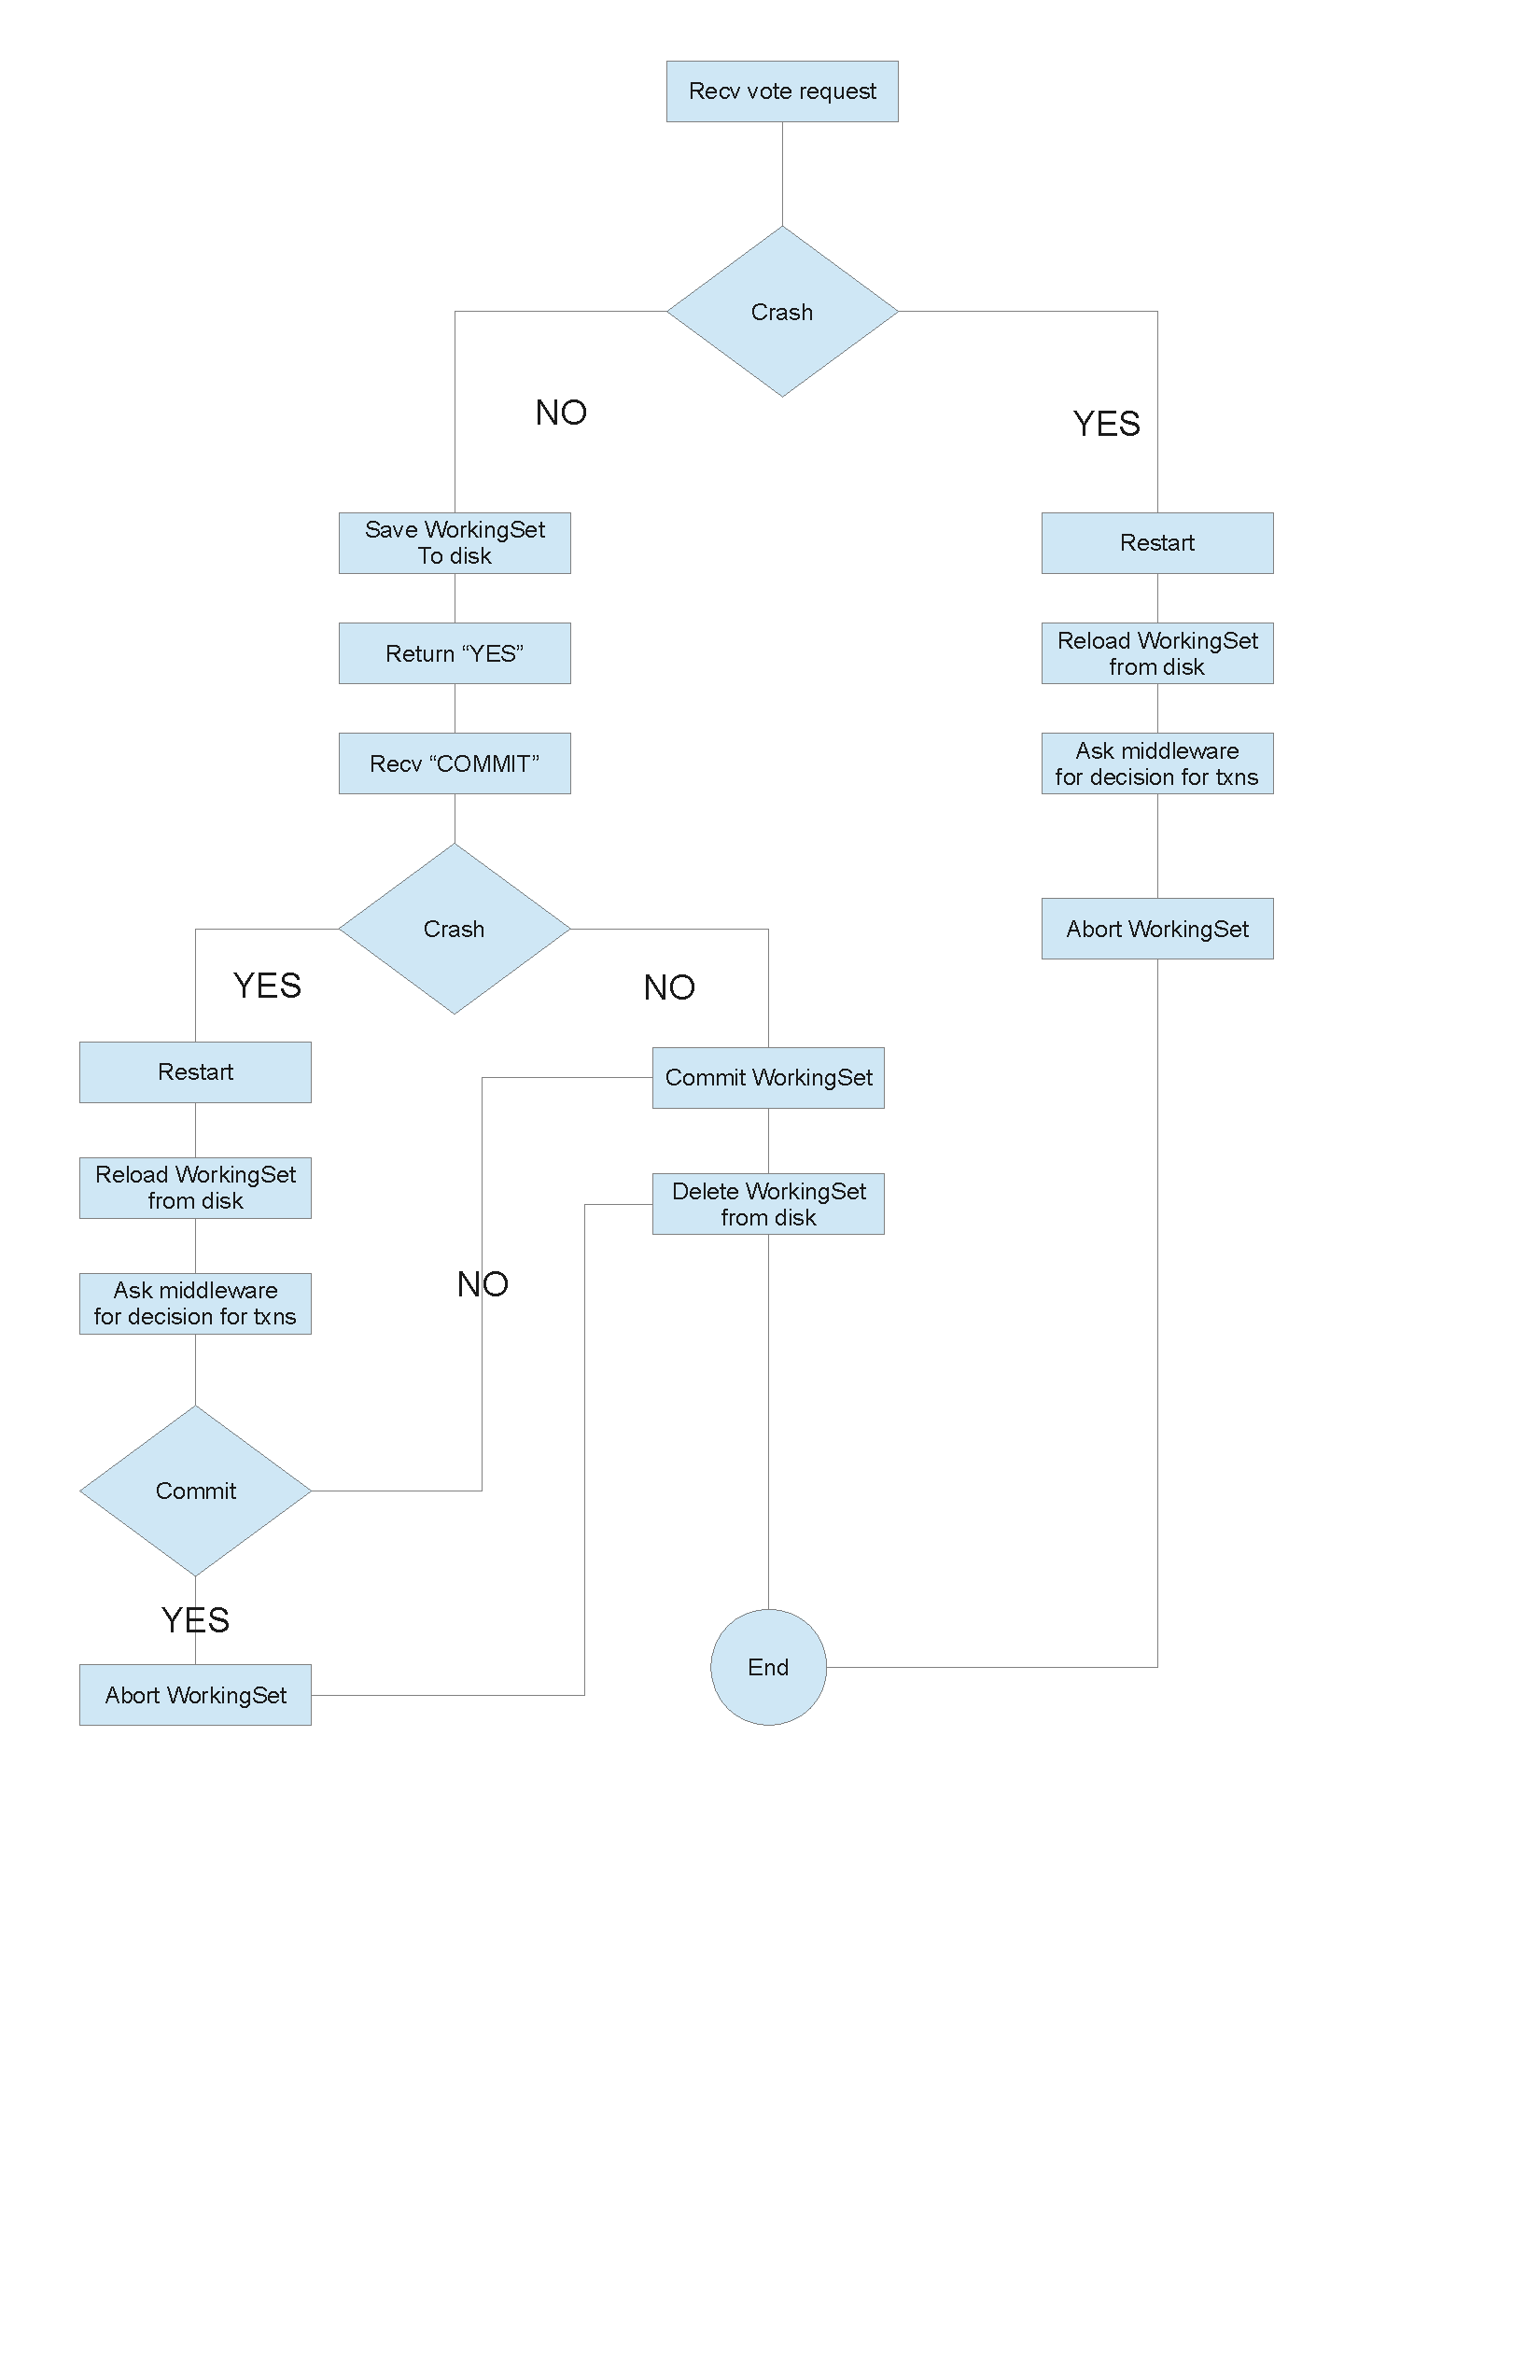
\includegraphics[scale=0.6]{2pc.pdf}
  \end{center}
\end{figure}

\begin{figure}[H]
  \caption{Two-phase commit (middleware view)}
  \label{fig:2pc-mw}

  \begin{center}
    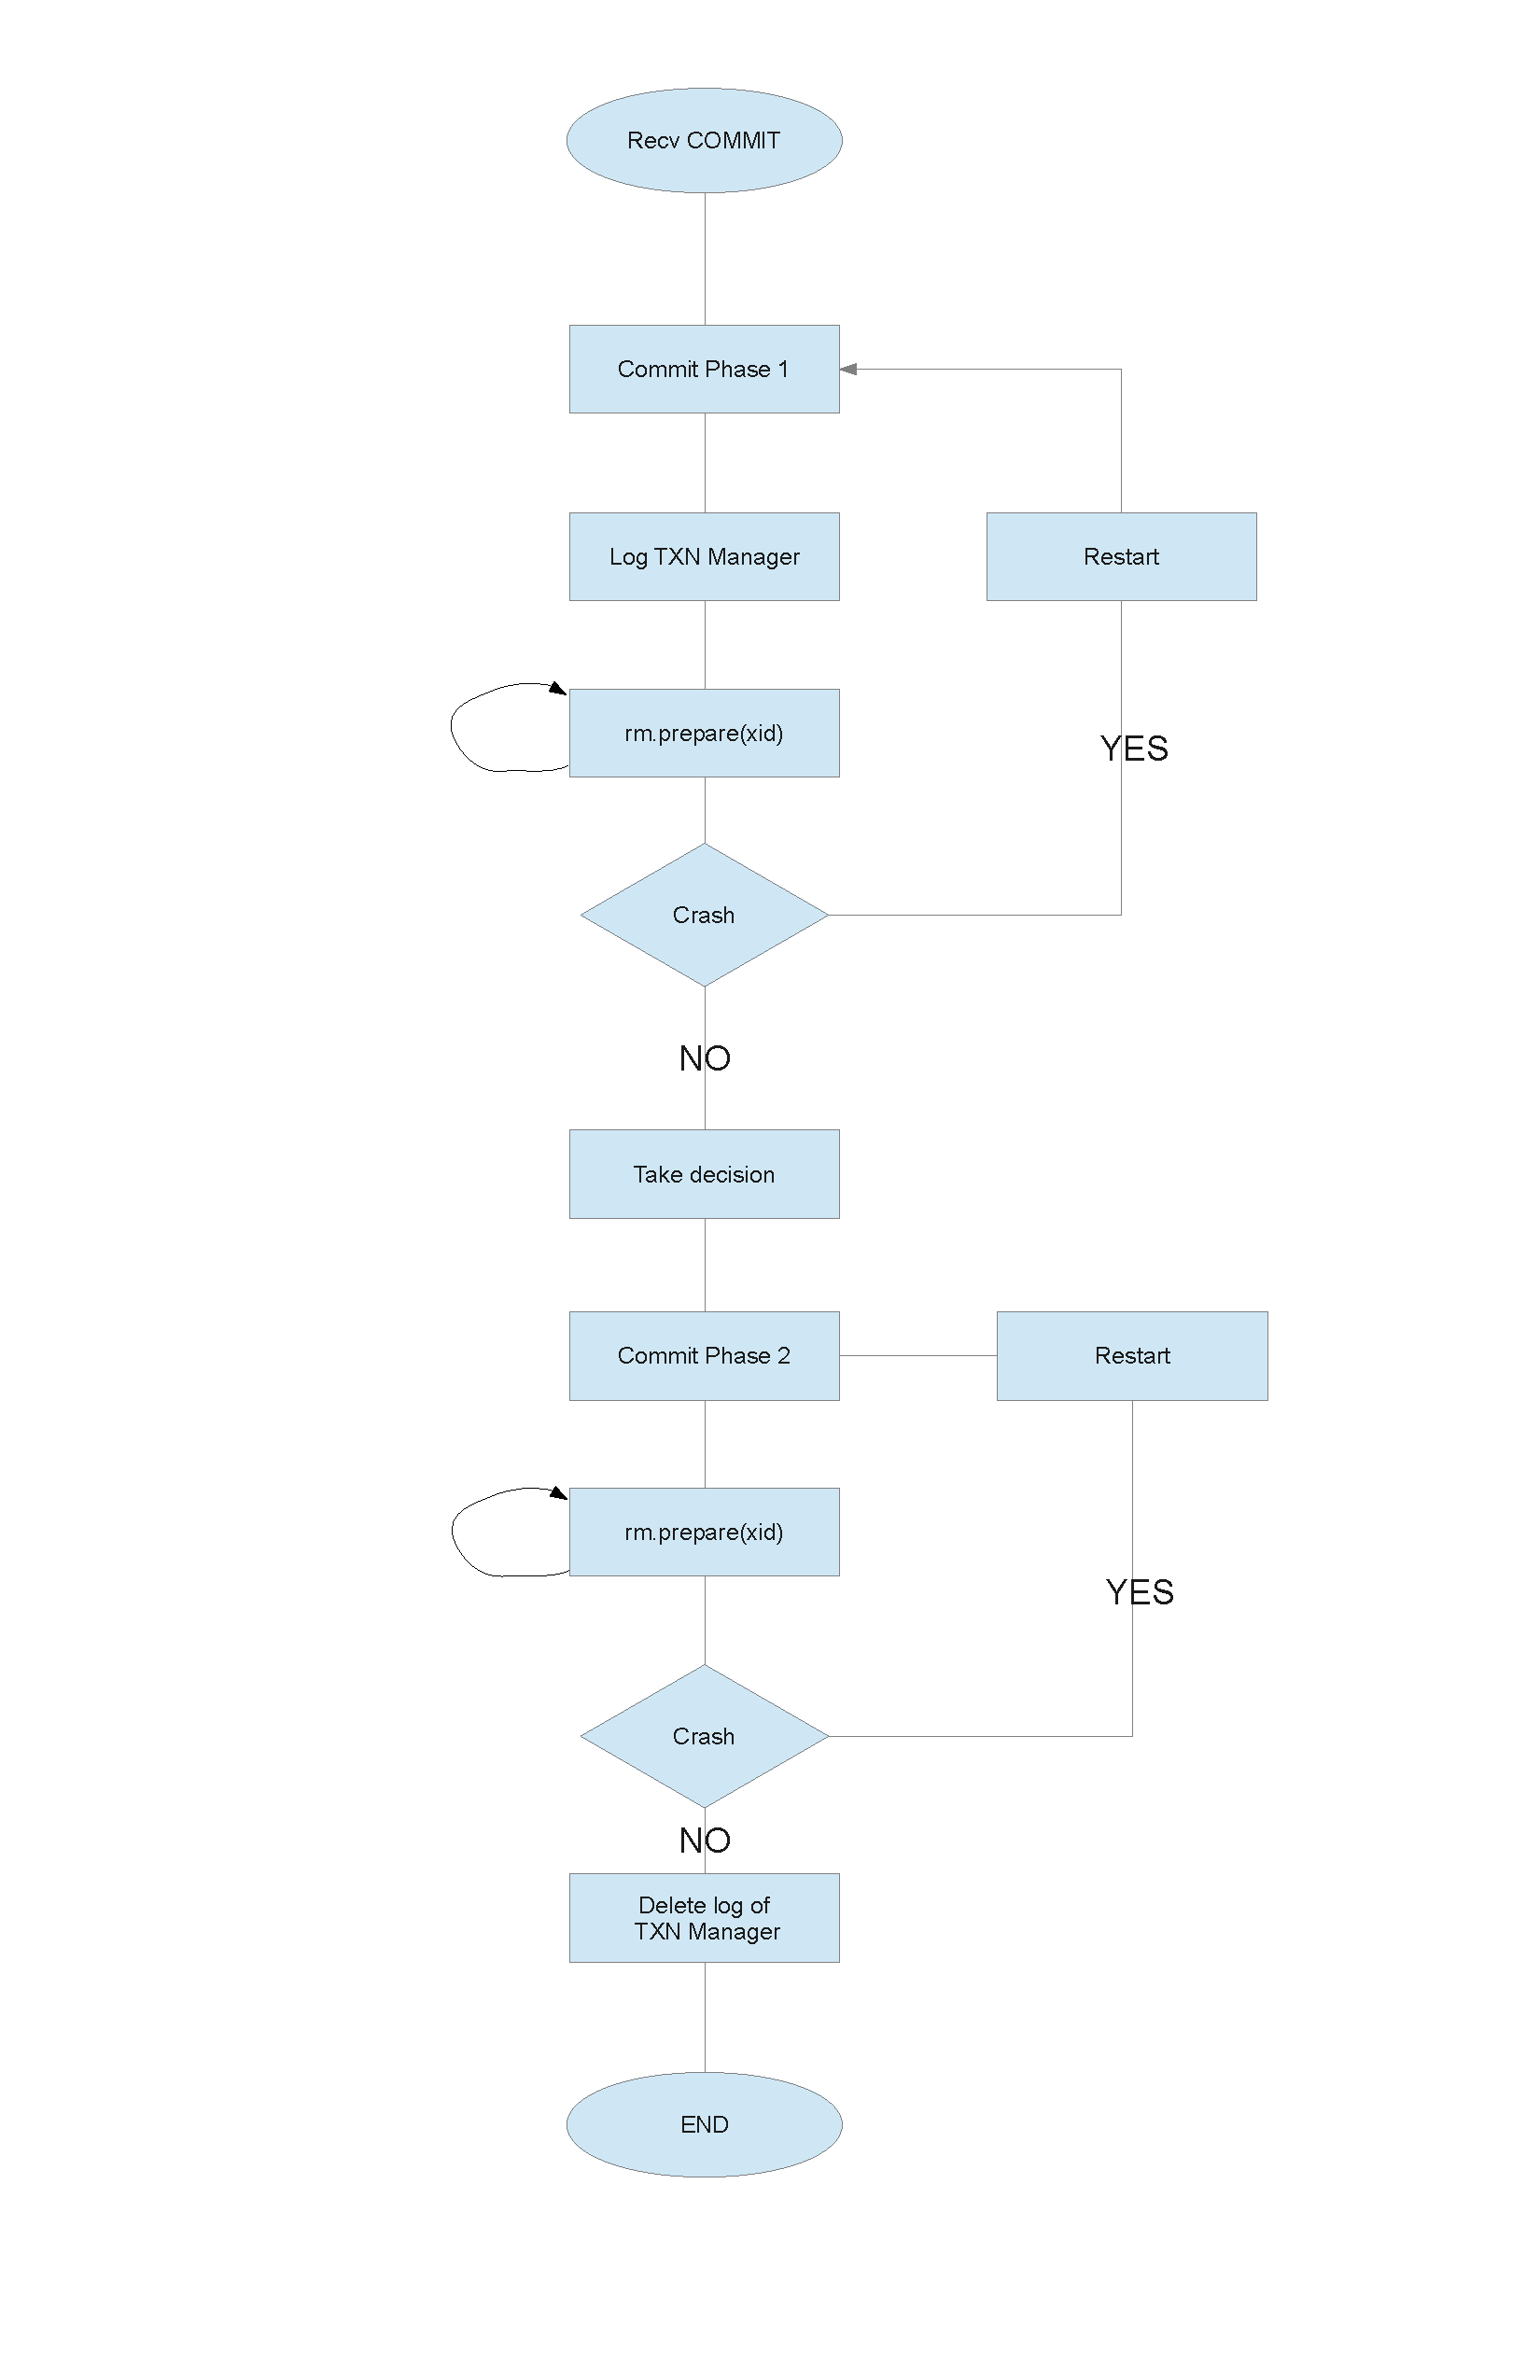
\includegraphics[scale=0.6]{2pc-mw.pdf}
  \end{center}
\end{figure}


\subsection{The Happy Path}

In the ideal scenario, without any failures, the two-phase commit
procedure goes like this:

\begin{itemize}
  \item A client asks to commit its transaction.
  \item The middleware receives this command and sends a vote request
    ({\it prepare}) to all resource managers involved in this
    transaction, asking if they can commit or not.
  \item All the resource managers write their working set to disk and
    give a positive response to the middleware.
  \item Since all resource managers responded affirmatively, the
    middleware sends a message to perform the commit operation.
  \item The resource managers apply the commands in their working sets
    to the data items.
  \item The working set copy on disk is deleted.
  \item The modified hash table is written to into the working copy
    and the master record is updated.
\end{itemize}

\subsection{Crash at a participant}

When a participant (i.e. a resource manager) crashes, either its
working set has been saved to disk (e.g. {\it /tmp/Group5/car\_123.ws})
or it hasn't.  If the working set doesn't exist, no recovery is
possible and the transaction will be aborted.

If the working set exists on disk, we load it into memory, and we
initiate the recovery procedure.  When a resource manager is started
in recovery mode, it has a reference to the middleware, and will ask
it what to do (i.e. abort or commit) with every transaction in the
working set.  Once the recovery procedure is completed, the resource
manager works as usual.

Here we describe what happens at different crash sites for a
participant:

\begin{itemize}
  \item {\bf Crash before saving working set:} no recovery is possible
    for this participant, and other participants in the transaction
    are instructed to abort.
  \item {\bf Crash after saving working set:} when the resource
    manager restarts, it'll query the middleware to know what to do
    with the transactions.  Because the RM hadn't sent its response,
    the middleware aborted the whole transaction, and thus the
    resource manager will abort.
  \item {\bf Crash after sending response:} the resource manager will
    query the middleware, and the middleware will tell it whether it
    has to commit or abort the transaction.
\end{itemize}


\subsection{Crash at the middleware}

Dealing with crashes in the middleware is a lot trickier than in a
resource manager, because it is the central hub of the whole
application.  Clients lose their links to the middleware during a
crash, and those links cannot be restored (the middleware doesn't know
about clients) automatically.  Clients need to reconnect to be able to
work again.

We handle crashes of the middleware during the two-phase commit
procedures in two scenarios.

The first scenario corresponds roughly to the first phase of the
two-phase commit; if the middleware crashes at anytime during that
phase (e.g. before sending vote requests, when some vote requests have
returned, when all vote requests have returned, etc.), during its
recovery procedure the middleware will send the vote request again.
On the resource manager side, the working set file will be overwritten
(no problem) and the response will be sent again.

The second scenario is when a decision has been taken (i.e. to commit
or to abort).  If the middleware crashes during that time, during
recovery, it'll re-send the decision to all the resource managers.
Again, on the resource manager side, the effect of receiving a
duplicate decision is benign; if the transaction had already been
processed, the new decision will be ignored, otherwise it'll be
processed.


\subsection{Information on recovery}

When a resource manager crashes and comes back up, it needs to query
the transaction manager through the middleware to know how to handle
the transactions in its working set.  As we saw in the {\it RMI}
section, resource managers do not have a reference to the middleware,
so how can they request that information?

One solution we considered was to have a watchdog process that would
periodically send a ping to the resource managers asking them if they
were interested in information on some transactions.  Keeping track of
who needed which information would be difficult, and sending all the
information to every resource manager would be wasteful.  We therefore
rejected this approach.

Instead, we elected to give a direct RMI reference to the middleware
when a resource manager boots in recovery mode.  This makes it fast,
easy and direct to obtain the information about the transactions.



\section{Implementation difficulties}

\subsection{The handling of customers}

Customers are handled inside the middleware; because the ItemManager
interface doesn't map well to customers, the middleware does not
implement that interface.  Consequently, customers cannot be handled
by the same code that handles the other resource managers.  This
causes code to be duplicated in many place to handle customers
properly.

Also, because the middleware has more responsibilities than the
resource managers, extra code must often be added.  Combined together,
this makes the code brittle and hard to modify.

\subsection{Internal vs. external modifications}

When we had to add new functionality (e.g. lock managers), we applied
the modifications directly inside the methods that already existed.
While this works and is relatively simple in principle, adding more
and more responsibilities to a single method makes them harder to
reason about, harder to test thoroughly and the primary task that a
method performs is clouded by the extra tasks that are interleaved
into the body of the function must perform and the relevant error
handling.

Perhaps a better approach would have been to use the decorator patter
to better separate the tasks into different classes so that the
original code could have been left unmodified.  However, due to the
uncertainty that such a design could be realized in a timely fashion,
we've opted to go for the simpler, but messier design.

\subsection{Code duplication}

Because the resource manager don't inherit from a superclass, but
implement an interface (which by definition cannot contain any
implementation), we found ourselves copy/pasting a lot of code that we
might have normally handled by writing a method in the parent class.



\subsection{Crashing the resource managers}

Crashing the resource managers proved a bit tricky when they were in
recovery mode; since they had a reference to the middleware, they had
a running non-daemon thread that prevented them the JVM from exiting,
even when calling {\it System.exit()}.  We found the solution (quite
by accident) online where a blogger recommended using the {\it
  Runtime.getRuntime().exit()} call to exit even when RMI references
were involved.  This fixed our problem.


\subsection{Unit testing}

It is nigh impossible to test automatically this
software; bringing up the whole system, populating the system with
data, making managers interact in different orders, testing each
individual feature and each combination of features, etc. would be
harder and longer than doing manual checking.

Some of the tests that we executed manually to ensure the correctness of the
implementation are detailed in the {\it presentation.pdf} slideshow available
in the project directory.


\section{Performance evaluation}

(Note: the following performance evaluation have been performed
without the code for two-phase commit.)

\subsection{Single client}

We evaluated the marginal performance of the system by executing read,
write and read/write operations on a single RM and on all three RMs.
We also ended transactions with both commits and aborts.  Because the
times to execute a single command were so low, we executed 50 commands
in total in each transaction.  The average latencies of 1000 measures
are given below in milliseconds.

\begin{tabular}{l|r|r}
  ~ & 1 RM & 3 RMs \\
  \hline
  Read + Commit  & 5.189131 & 6.955100 \\
  Read + Abort   & 5.434654 & 7.042538 \\
  Write + Commit & 12.987475 & 10.064491 \\
  Write + Abort  & 12.985847 & 10.060301 \\
  Read/Write + Commit & 7.466607 & 9.073547 \\
  Read/Write + Abort  & 7.465912 & 9.209547 \\
\end{tabular}

A few surprising facts emerge from these figures:

\begin{itemize}
  \item When only writes are concerned, accessing the 3 RMs is faster
    than accessing only one.
  \item Though they have more work to perform (i.e. executing the
    buffered commands), the commit transactions are usually a little
    faster than the abort transactions.
\end{itemize}

A fact that can only be observed by looking at the raw data is how the
system gets faster as more commands are sent to the system; the first
few transactions execute in ~30ms before reaching numbers usually
below 10ms.  We attribute this to the Java JIT that warms up and
starts optimizing the RM methods after they've been ran a sufficient
number of times.

\subsection{Multiple clients}

For our performance evaluation, we used the following parameters:

\begin{itemize}
\item A fixed number of clients was selected (5, 10, 25, 50, 100, 200,
  500, and 1000)
\item A sleep interval (in milliseconds) between commands was selected
  (1000, 500, 250, 100, 50, 10)
\end{itemize}

For every combination of parameters, the following process was
executed:

\begin{enumerate}
\item The servers were started with empty hash tables.
\item The RMs were populated with 1000 cities (for cars
  and hotels), 1000 flights and 1000 customers.
\item Random commands were executed and committed by the clients for
  60 seconds.
\item The latency times were recorded in a file.
\end{enumerate}

The tests were ran on a Intel i7-3770S 3.10GHz.  To obtain times that
reflected the performance of the application, the server, RMs and
clients were all running on the same machine.  We took the arithmetic
average of the latencies and obtained the chart below.  From this
chart, we can make a few observations:

\begin{itemize}
\item The number of clients has a bigger impact on performance than
  the delay between commands
\item The latency time does not grow linearly with the number of
  clients.
\end{itemize}

Also, not apparent in the chart, the number of deadlocks increased
sharply as the number of clients increased, which is to be expected as
more clients will randomly select the same resource to access.

Finally a chart showing the cumulative distribution function of the
latency times is shown.

\begin{center}
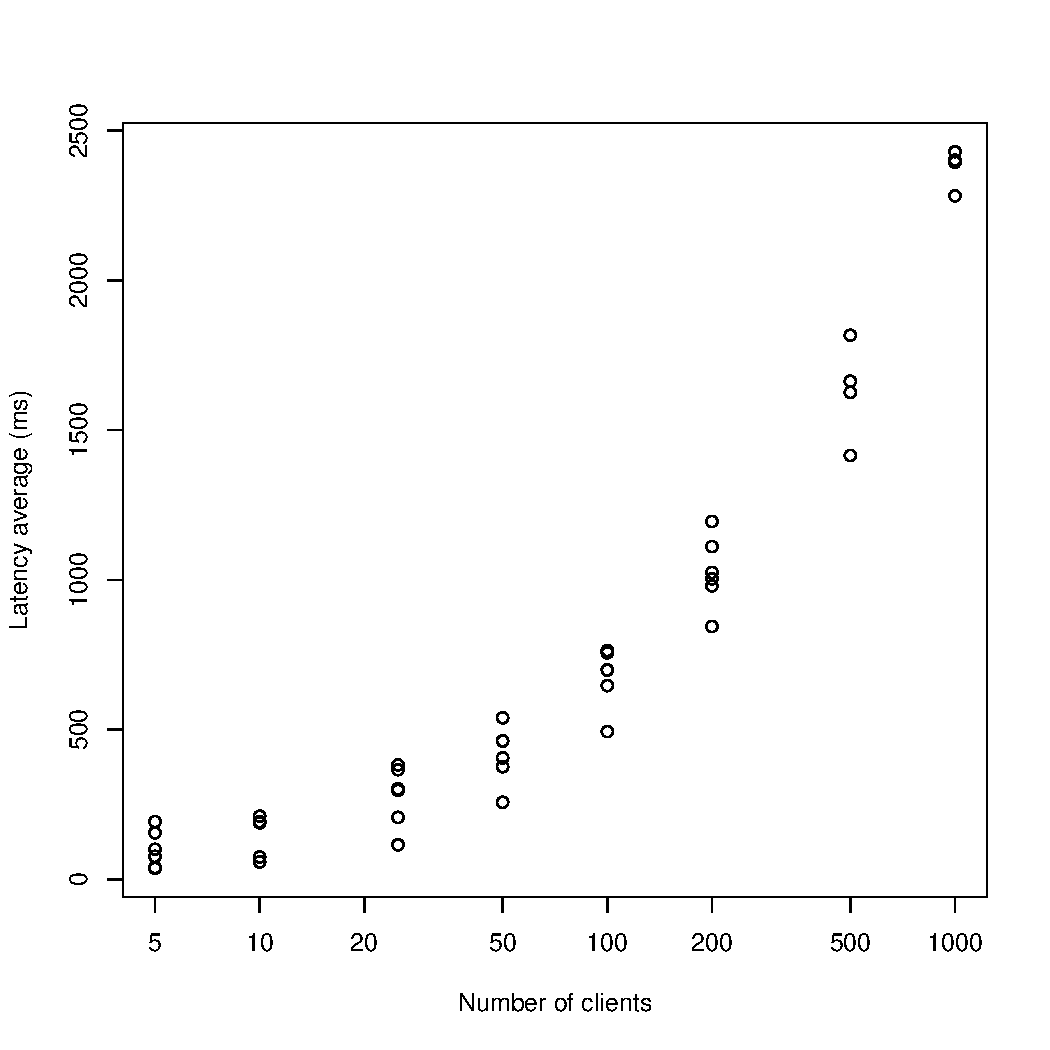
\includegraphics[scale=0.6]{avgs.pdf}
\\
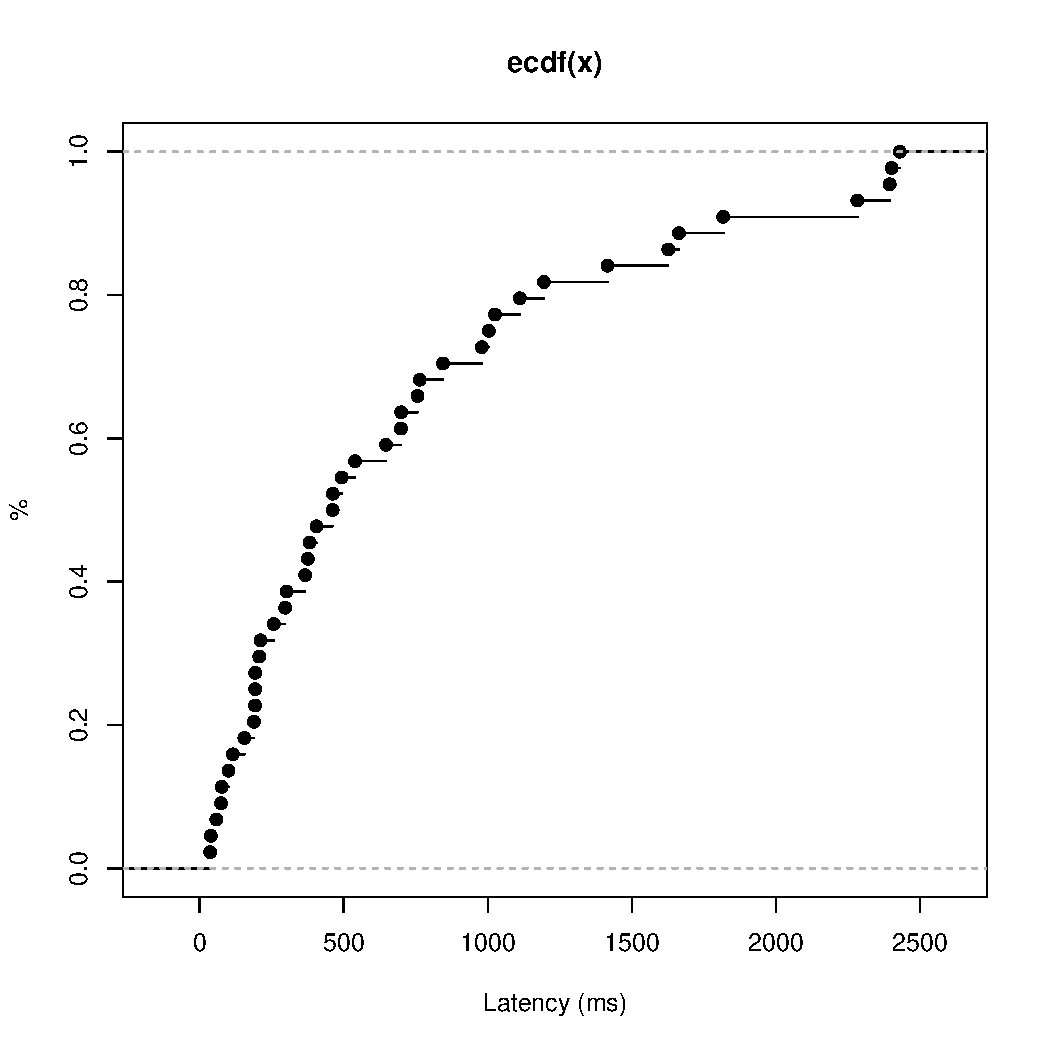
\includegraphics[scale=0.6]{cdf.pdf}
\end{center}


\end{document}
